\usetikzlibrary{positioning,shapes,arrows}
% Define block styles
\tikzstyle{decision} = [diamond, draw, fill=blue!20, 
    text width=5.5em, text badly centered, node distance=3cm, inner sep=0pt]
\tikzstyle{block} = [rectangle, draw, fill=blue!20, 
    text width=5em, text centered, rounded corners, minimum height=4em]
\tikzstyle{line} = [draw, -latex']
\tikzstyle{cloud} = [draw, ellipse,fill=red!20, node distance=3cm,
    minimum height=2em]

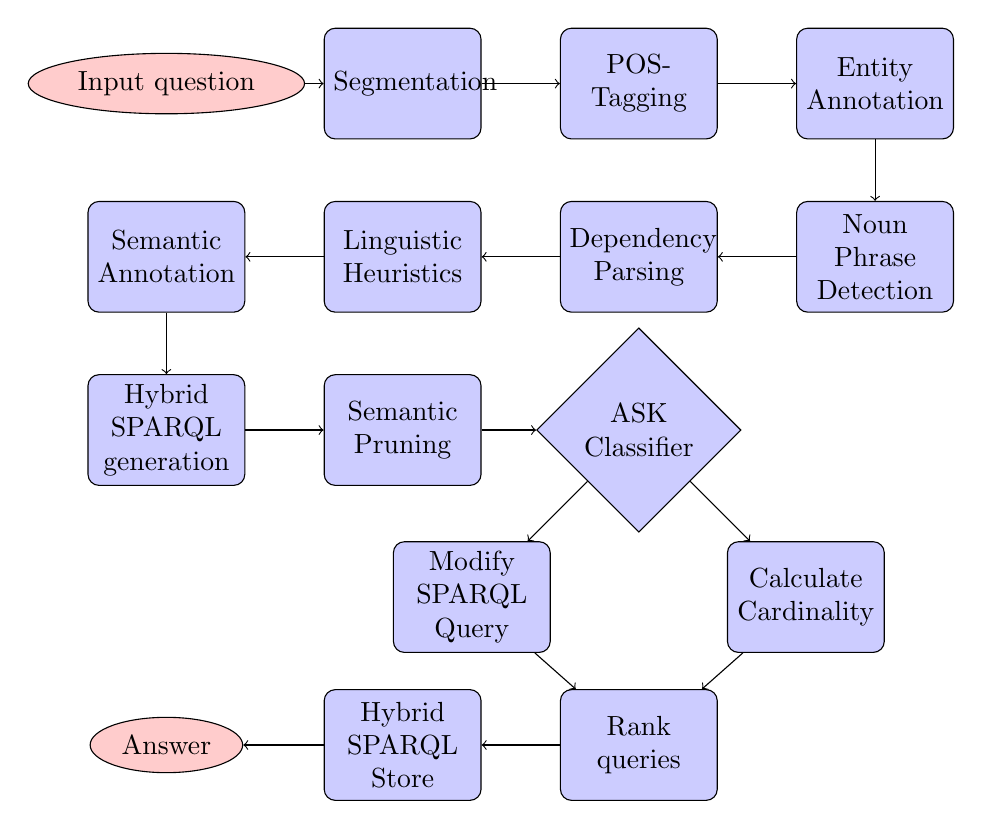
\begin{tikzpicture}[->,node distance = 3cm, auto]
    % Place nodes
    \node [cloud] (question) {Input question};
    \node [block, right of=question] (segmentation) {Segmentation};
    \node [block, right of=segmentation] (pos) {POS-Tagging};
    \node [block, right of=pos] (entityannotation) {Entity Annotation};
    \node [block, below of=entityannotation, node distance=2.2cm] (nounphrasedetection) {Noun Phrase Detection};
    \node [block, left of=nounphrasedetection] (dependency) {Dependency Parsing};
    \node [block, left of=dependency] (ling_heu) {Linguistic Heuristics};
    \node [block, left of=ling_heu] (sem_anno) {Semantic Annotation};
    \node [block, below of=sem_anno,node distance=2.2cm] (sparql) {Hybrid SPARQL generation};
    \node [block, right of=sparql] (sem_pruning) {Semantic Pruning};
    \node [decision, right of=sem_pruning] (classify) {ASK Classifier};
    \node [block, below left of=classify] (mod_ask) {Modify SPARQL Query};
    \node [block, below right of=classify] (calc_card) {Calculate Cardinality};
    \node [block, below of=classify,  node distance=4cm] (rank) {Rank queries};
    \node [block, left of=rank] (sparql_fire) {Hybrid SPARQL Store};
    \node [cloud, left of=sparql_fire] (answer) {Answer};
    %\node [decision, below of=evaluate] (decide) {is best candidate better?};
    % Draw edges
    \draw[->]  (question) -- (segmentation);
    \draw[->]  (segmentation) -- (pos);
    \draw[->]  (pos) -- (entityannotation);
    \draw[->]  (entityannotation) -- (nounphrasedetection);
    \draw[->]  (nounphrasedetection) -- (dependency);
    \draw[->]  (dependency) -- (ling_heu);
    \draw[->]  (ling_heu) -- (sem_anno);
    \draw[->]  (sem_anno) -- (sparql);
    \draw[->]  (sparql) -- (sem_pruning);
    \draw[->]  (sem_pruning) -- (classify);
    \draw[->]  (classify) -- (mod_ask);
    \draw[->]  (classify) -- (calc_card);
    \draw[->]  (mod_ask) -- (rank);
    \draw[->]  (calc_card) -- (rank);
    \draw[->]  (rank) -- (sparql_fire);
    \draw[->]  (sparql_fire) -- (answer);


   % \path [line] (decide) -| node [near start] {yes} (update);
   % \path [line] (update) |- (identify);
   %    \path [line] (decide) -- node {no}(stop);
\end{tikzpicture}